\documentclass[10pt,a4paper,oneside]{report}             % Single-side
%\documentclass[12pt,a4paper,twoside,openright]{report}  % Duplex

%\PassOptionsToPackage{chapternumber=Huordinal}{magyar.ldf}
\usepackage{bm}
\usepackage{amsmath}
\usepackage{amssymb}
\usepackage{enumerate}
\usepackage[thmmarks]{ntheorem}
\usepackage{graphics}
\usepackage{epsfig}
\usepackage{listings}
\usepackage{color}
\usepackage{algorithm}
\usepackage{algorithmic}
\usepackage{csquotes}
\usepackage{lastpage}
\usepackage{anysize}
\usepackage{sectsty}
\usepackage{setspace}  % Ettol a tablazatok, abrak, labjegyzetek maradnak 1-es sorkozzel!
\usepackage[hang]{caption}
\usepackage{hyperref}
\usepackage[english]{babel}
\usepackage{fontspec}
\usepackage{textcomp}
\usepackage{subcaption}
\usepackage{titlesec, blindtext, color}
\usepackage{fancyhdr}
\usepackage{lastpage}
\usepackage{todonotes}
\usepackage{graphicx}
\usepackage{tikz}
\usepackage{subcaption}
\usepackage{float}
\usepackage{listings}
\usepackage{xcolor}
\usepackage[sorting=none, backend=biber]{biblatex}
\addbibresource{bib.bib}
\lstloadaspects{formats}

\lstdefineformat{C++}{%
	\{=\newline\string\newline\indent,%
	\}=[;]\newline\noindent\string\newline,%
	\};=\newline\noindent\string\newline,%
	;=[\ ]\string\space}

\definecolor{commentgreen}{RGB}{2,255,10}
\definecolor{eminence}{RGB}{255,150,10}
\definecolor{weborange}{RGB}{255,10,0}
\definecolor{frenchplum}{RGB}{129,20,83}

\setlength{\headheight}{14.5pt}

\lstset {
	language=C++,
	frame=tb,
	tabsize=4,
	showstringspaces=false,
	numbers=left,
	%upquote=true,
	keywordstyle=\color{eminence},
	morestring=[b][\color{weborange}]__,
	morestring=[b][\color{weborange}]",
	basicstyle=\scriptsize\ttfamily, % basic font setting
	stringstyle=\scriptsize\sffamily, 	 			% typewriter type for strings
	showstringspaces=false,  
	emph={int,char,double,float,unsigned,void,bool,short,long,uchar,uchort,uint,ulong,dim3},
	emphstyle={\color{blue}},
	% keyword highlighting
	classoffset=1, % starting new class
	otherkeywords={>,<,-,!,=,~,+,*},
	morekeywords={>,<,-,!,=,~,+,*},
	morecomment=[f][\color{commentgreen}][0]{//},
	commentstyle=\color{commentgreen},
	keywordstyle=\color{eminence},
	classoffset=0,
}

%--------------------------------------------------------------------------------------
% Main variables
%--------------------------------------------------------------------------------------
\newcommand{\vikauthor}{Márton Szemenyei}
\newcommand{\viktitle}{VATEM3}
\newcommand{\vikdept}{}
\newcommand{\vikdoktipus}{User Manual}

%--------------------------------------------------------------------------------------
% Page layout setup
%--------------------------------------------------------------------------------------
% we need to redefine the pagestyle plain
% another possibility is to use the body of this command without \fancypagestyle
% and use \pagestyle{fancy} but in that case the special pages
% (like the ToC, the References, and the Chapter pages)remain in plane style

\pagestyle{plain}
\setlength{\parindent}{0pt} % 
\setlength{\parskip}{8pt plus 3pt minus 3pt} % 
%\setlength{\parindent}{12pt} % 
%\setlength{\parskip}{0pt}    % 

\marginsize{35mm}{25mm}{15mm}{15mm} % anysize package
\setcounter{secnumdepth}{0}
\sectionfont{\large\upshape\bfseries}
\setcounter{secnumdepth}{2}

%--------------------------------------------------------------------------------------
%	Setup hyperref package
%--------------------------------------------------------------------------------------
\hypersetup{
    pdftitle={\viktitle},        % title
    pdfauthor={\vikauthor},    % author
    pdfsubject={\vikdoktipus}, % subject of the document
    pdfcreator={\vikauthor},   % creator of the document
    pdfkeywords={VATEM3, Video Assisted Measurement, User Manual},    % list of keywords
    pdfnewwindow=true,         % links in new window
    colorlinks=true,           % false: boxed links; true: colored links
    linkcolor=black,           % color of internal links
    citecolor=black,           % color of links to bibliography
    filecolor=black,           % color of file links
    urlcolor=black             % color of external links
}

%--------------------------------------------------------------------------------------
%	Some new commands and declarations
%--------------------------------------------------------------------------------------
\newcommand{\code}[1]{{\upshape\ttfamily\scriptsize\indent #1}}

% define references
\newcommand{\figref}[1]{\ref{fig:#1}.}
\renewcommand{\eqref}[1]{(\ref{eq:#1})}
\newcommand{\listref}[1]{\ref{listing:#1}.}
\newcommand{\sectref}[1]{\ref{sect:#1}}
\newcommand{\tabref}[1]{\ref{tab:#1}.}

\newcommand*{\img}[1]{%
	\raisebox{-.02\baselineskip}{%
		\includegraphics[
		height=\baselineskip,
		width=\baselineskip,
		keepaspectratio,
		]{#1}%
	}%
}

\DeclareMathOperator*{\argmax}{arg\,max}
%\DeclareMathOperator*[1]{\floor}{arg\,max}
\DeclareMathOperator{\sign}{sgn}
\DeclareMathOperator{\rot}{rot}
\definecolor{lightgray}{rgb}{0.95,0.95,0.95}

\newcommand{\hsp}{\hspace{20pt}}
\titleformat{\chapter}[hang]{\Huge\bfseries}{\thechapter\hsp}{0pt}{\Huge\bfseries}
\titlespacing*{\chapter}{0pt}{0pt}{40pt}


\author{\vikauthor}
\title{\viktitle}
%--------------------------------------------------------------------------------------
%	Setup captions
%--------------------------------------------------------------------------------------
\captionsetup[figure]{
%labelsep=none,
%font={footnotesize,it},
%justification=justified,
width=.9\textwidth,
aboveskip=10pt}

\renewcommand{\captionlabelfont}{\small\bf}
\renewcommand{\captionfont}{\footnotesize\it}

\fancypagestyle{plain}{%
	\fancyhf{}
	\renewcommand{\footrulewidth}{1pt}
	\chead{\viktitle ~- \vikdoktipus}
	\lfoot{\thepage/\pageref{LastPage}} %/\pagetotal
	\rfoot{\leftmark}
}
\pagestyle{plain}

\pagestyle{fancy}
\renewcommand{\chaptermark}[1]{\markboth{\MakeUppercase{#1}}{}}
\fancyhf{}
\chead{\viktitle}
\lfoot{\thepage/\pageref{LastPage}} %/\pagetotal
\rfoot{\leftmark}
\renewcommand{\footrulewidth}{1pt}

%--------------------------------------------------------------------------------------
% Table of contents and the main text
%--------------------------------------------------------------------------------------
\begin{document}

\singlespacing

%--------------------------------------------------------------------------------------
%	The title page
%--------------------------------------------------------------------------------------
\begin{titlepage}
\begin{center}
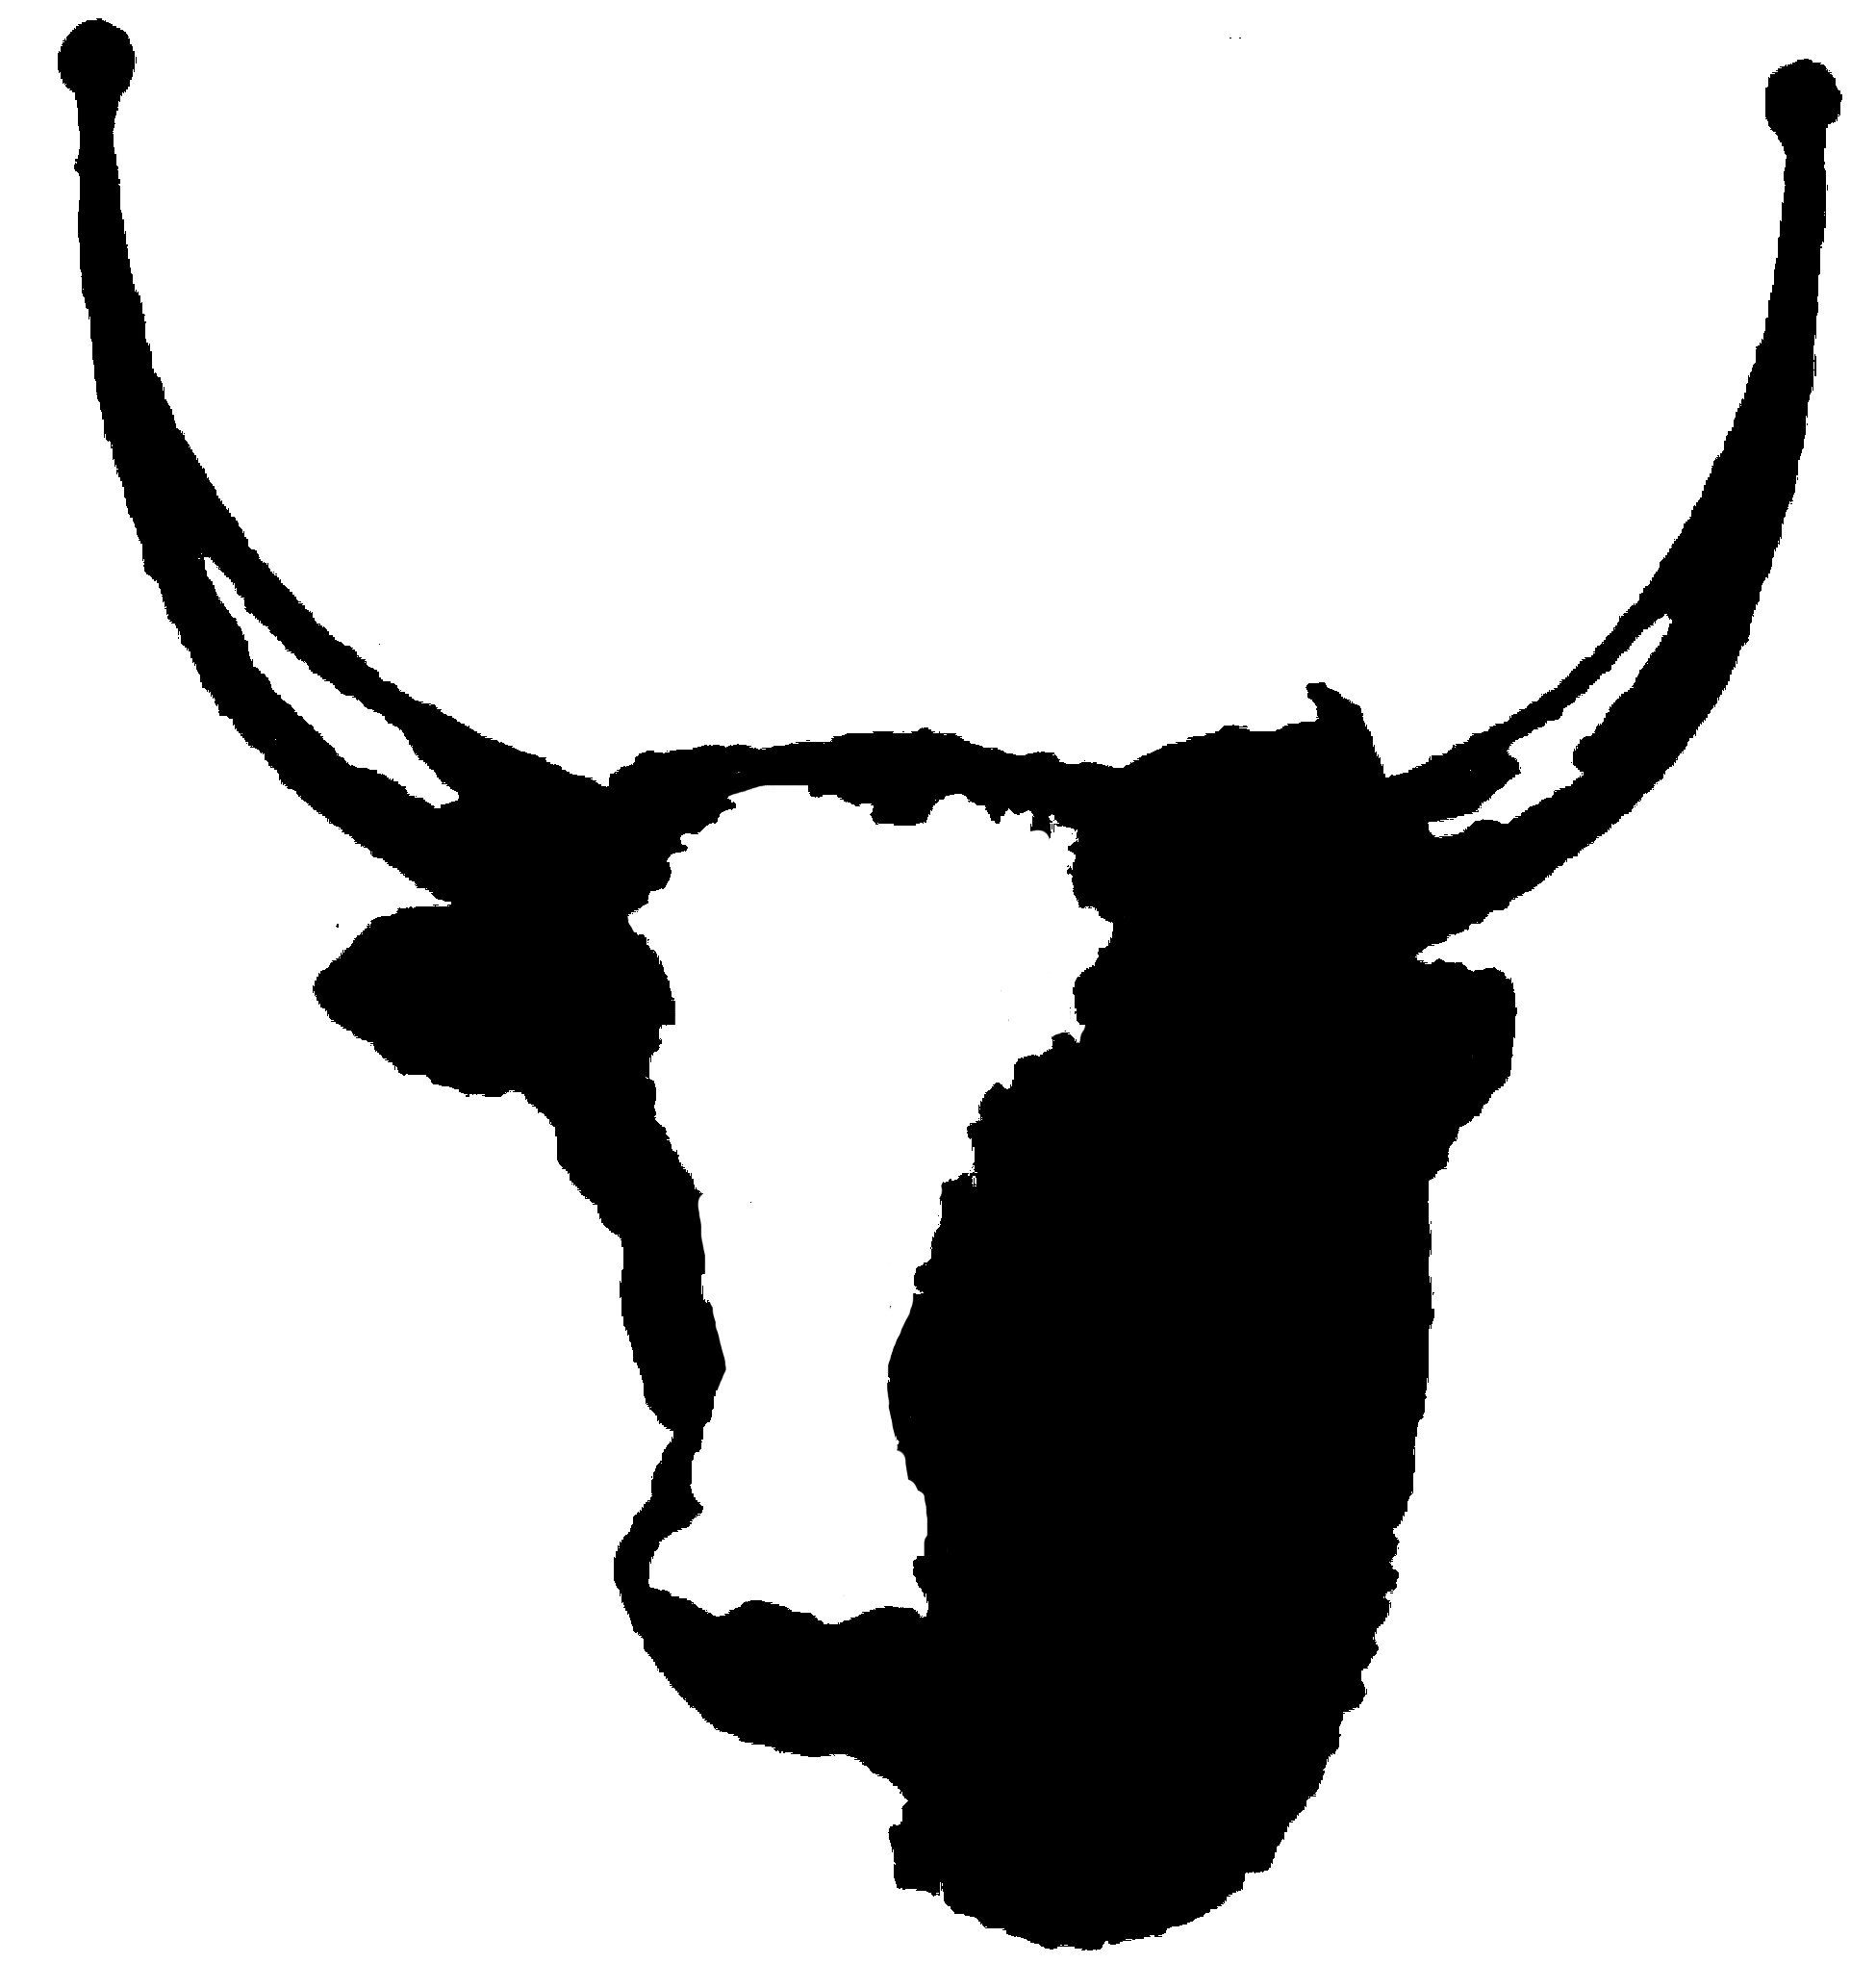
\includegraphics[width=60mm,keepaspectratio]{../VAM/icons/ikon01.png}\\
\vspace{0.3cm}
\textbf{University of Veterinarian Sciences}\\
%\textmd{Faculty of Electrical Engineering and Informatics}\\
\textmd{\vikdept}\\[5cm]

\vspace{0.4cm}
{\huge \bfseries \viktitle}\\[0.8cm]
\textsc{\Large \vikdoktipus}\\[2cm]
\textsc{\Large \vikauthor}\\[6cm]

\vfill
{\large \today}
\end{center}
\end{titlepage}

%\pagenumbering{arabic}

%--------------------------------------------------------------------------------------
% tartalom, ábra és táblázatjegyzék
%--------------------------------------------------------------------------------------
\singlespacing
\tableofcontents\thispagestyle{fancy}


\chapter{Basic Usage}

Welcome to the VATEM3 User Manual. This document will guide you in the basic usage of the Video AssisTEd Measurement application. This chapter covers the basic usage of the software, including importing videos and creating or importing still images of the animals to be measured, creating schemas, marking still images, and finally, exporting data. More advanced usage, such as camera calibration, automatic still detection, planimetrics and morphometrics will be covered in later chapters. 
 
\section{Projects}

Upon opening the software you will be greeted by the \textbf{Project Window}. This screen aims to give you a general overview of the stage of completion of your measurement project. Stages with a green checkmark are completed, while those with a red cross sign are not completed. To make newer stages available, please complete all previous stages.

\begin{figure}[H]
	\centering
	\begin{subfigure}{\textwidth}
		\centering 
		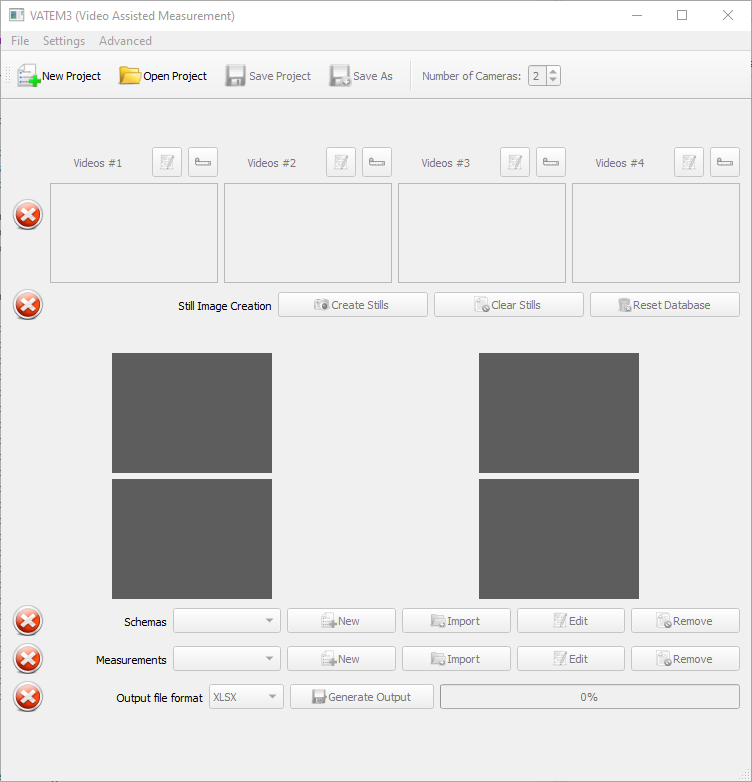
\includegraphics[width=0.75\textwidth]{./images/MW1.png}
	\end{subfigure}
	\caption[]
	{\small  The Project Window.}
\end{figure} 

You first step is to create a new project, or open an existing one by clicking the appropriate button in the toolbar at the top of the window. Upon creating a new project you will be asked to enter its name. By default projects are saved into the \textit{"Documents/VATEM3/<Project Name>"} folder and have the extension of \textit{.vamproj}. You can change the default project folder in the \textbf{Advanced menu}.

\begin{figure}[H]
	\centering
	\begin{subfigure}{\textwidth}
		\centering 
		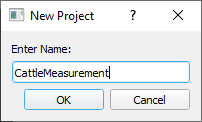
\includegraphics[width=0.25\textwidth]{./images/NewProj.png}
	\end{subfigure}
	\caption[]
	{\small  Creating a project.}
\end{figure} 

\subsection{Setting the number of videos}

The next step is setting the number of videos/cameras your project uses. VATEM3 supports projects between 1 and 4 cameras that observe the animals from different angles or positions. By changing the number of videos, you will se the user interface reacting by adding the appropriate number of user interface elements.

\section{Adding videos}

The next step is adding the videos to your project by opening the \textbf{Video Interface}. You can do this separately for each camera by clicking the \textbf{Add} \img{../VAM/Icons/1462036180_list-add.png} button below the corresponding empty list. Here, you can browse your computer, and select multiple video files, and order them as you please. \textbf{You need to select at least one video file for each camera!}

\begin{figure}[H]
	\centering
	\begin{subfigure}{\textwidth}
		\centering 
		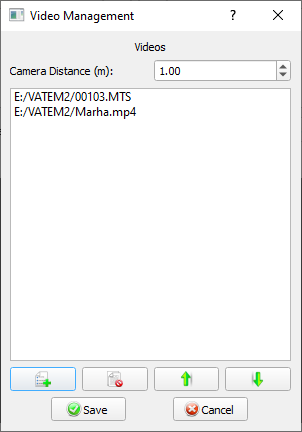
\includegraphics[width=0.35\textwidth]{./images/AddVid.png}
	\end{subfigure}
	\caption[]
	{\small  The Video Interface.}
\end{figure} 

\subsection{Camera distance}

For the second, and higher cameras, the \textbf{Video Interface} will have an extra element, allowing you to set the \textit{Camera Distance}. This value is necessary to use the \textit{Automatic Measurement Correction} feature of the software. In this setting you need to set the distance between the camera and the etalon/reference measurement object. You will be able to define a measurement that signals the distance between the etalon/reference object and the animal at a later stage. NOTE: This feature is only available for cameras \# 2 an up. 

\section{Still database}

The next task is to take still images on animals using the videos imported in the previous stage. To do this, open the \textbf{Still Window} by clicking on the \textit{Create Stills} button. In this window, you can play and pause each video independently, or at the same time by using the \textit{Frame Lock} setting the the toolbar. The toolbar also contains a \textit{Deinterlace} option for interlaced videos, and you can also toggle the window (\img{../VAM/Icons/if_tile_windows_horizontally_16x16_10026.png}) to arrange your videos vertically or horizontally.

The video players allow you to play or pause the videos, skip to the previous/next videos (\img{../VAM/Icons/1462036208_Skip-Backward.png} \img{../VAM/Icons/1462036208_Skip-Forward.png} buttons), and navigate forward/backward frame by frame (\img{../VAM/Icons/1462036188_Fast-Backward.png} and \img{../VAM/Icons/1462036188_Fast-Forward.png} buttons).

\begin{figure}[H]
	\centering
	\begin{subfigure}{\textwidth}
		\centering 
		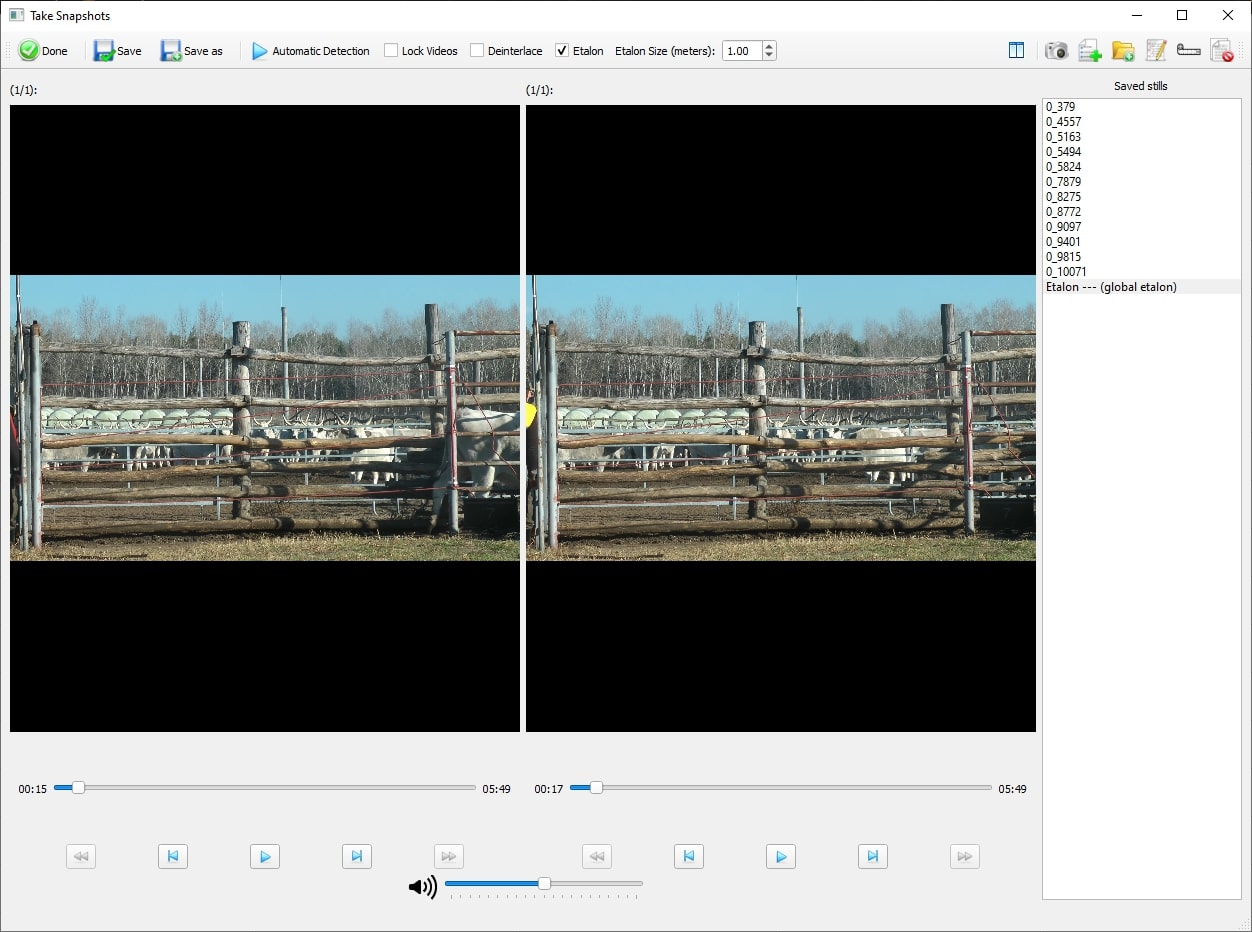
\includegraphics[width=0.95\textwidth]{./images/VideoW.jpg}
	\end{subfigure}
	\caption[]
	{\small  The Still Window.}
\end{figure} 

The \textbf{Project Window} allows you to clear all still images previously created in the database, while you can also reset the database, which also clears all videos added in the previous stage.

\subsection{Taking snapshots}

To create a still image, it is recommended that you pause all videos at the desired frame. Then, by clicking the \textit{Take Snapshot} \img{../VAM/Icons/1462024260_Camera.png} button, you can take a still image from all videos simultaneously. The program will then attempt to find a QR or barcode in each of the images that contains the ID of the animal. Regardless of the results, the software will prompt you to enter an ID. You can change the ID of any animal by selecting the animal from the side list, and clicking the \textit{Edit} \img{../VAM/Icons/1462036358_edit.png} button, or delete them completely using the \textit{Remove} \img{../VAM/Icons/1462036183_document-delete3.png} button.

\subsection{Setting global etalon}

Etalon images are used to provide the software with a known reference. When taking the video it is important to have at least one etalon shown to all cameras. Etalon images only have two measurement points, which define one distance. The size of the etalon can be set for each etalon still image separately using the toolbar.

To mark a still image as etalon, select the image from the side list, and click the \textit{Etalon} checkbox in the top toolbar. Note, that the state of this checkbox changes automatically to reflect the etalon status of the \textit{currently selected image}. While you can mark multiple images as etalon, the software will only use the one marked as the \textit{Global Etalon} for the measurements. To set a still image as the global etalon, select a still that has already been marked as etalon, and click the \textit{Set Global Etalon} \img{../VAM/Icons/1462455465_centimeter.png} button in the top right. If successful, a visual indicator will appear in the list.

\subsection{Open images for stills} \label{sec:openStill}

If you already have still images that you want to add to the database, you can do that by clicking the \textit{Open Stills} \img{../VAM/Icons/1462367694_folder_open-add2.png} button. This will prompt a file selection dialog for each camera. \textbf{NOTE: You will see as many file selection dialogs, as you have cameras, so select only still image belonging to camera \# 1 in the first dialog, and so on.}

Once you have selected still images for all cameras, the \textbf{Still Pairing Window} will pop up, allowing you to select which stills from the different cameras belong to the same animal. You can do this by selecting a still from each input list, and adding them to the output list on the right. This action will also run the QR code detection, and prompt you to enter an ID. You can also remove paired stills and pair them again, if needed. NOTE: At this stage, you can create incomplete entries (i.e.: animals that are missing stills from some cameras), but to complete the still creation stage, these incomplete entries have to be completed. 

\begin{figure}[H]
	\centering
	\begin{subfigure}{\textwidth}
		\centering 
		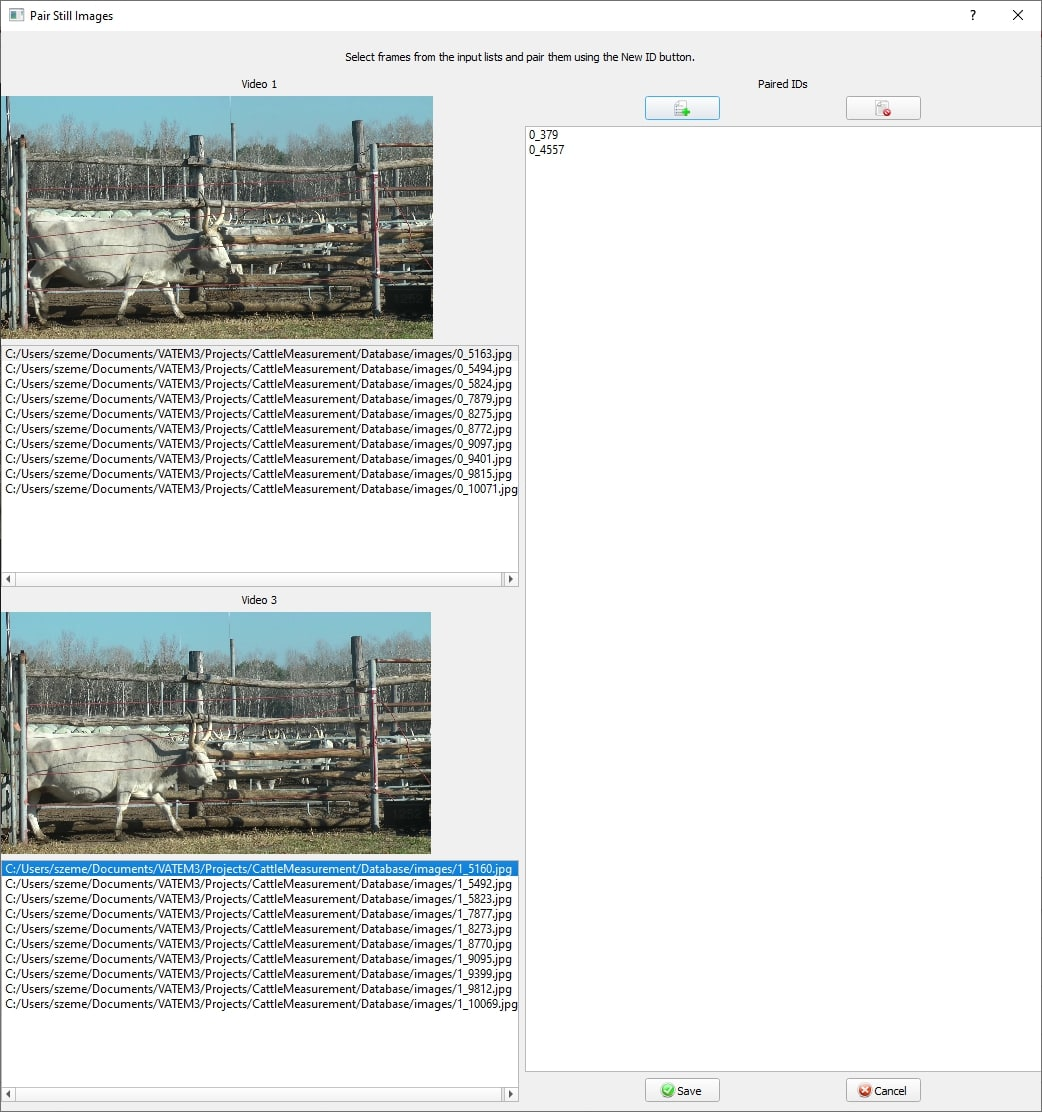
\includegraphics[width=0.65\textwidth]{./images/PairStill.jpg}
	\end{subfigure}
	\caption[]
	{\small  The Still Pairing Window.}
\end{figure} 

By clicking the \textit{Save} \img{../VAM/Icons/1462036176_save_accept.png} button, the opened stills will be added to the database.

\subsection{Complete stills} \label{sec:compStill}

If you have incomplete stills in your database, you can complete them by performing the following steps:
\begin{enumerate}
	\item Navigate the videos to the desired positions  and pause them.
	\item Select the incomplete still from the right side list.
	\item Click the \textit{Complete Still} \img{../VAM/Icons/1462024271_New_image.png} button, which will create new stills for all cameras that were marked as missing.
\end{enumerate}

\section{Schemas}

The next stage following the still creation is the \textbf{Schema Definition}. \textit{Schemas} contain the definition of marker points and the measurements made up by these points.

A single project may contain multiple schemas, if you wish to mark the same set of animals using different points or measurements. In the \textbf{Project Window}, you can add and import schemas to your project, whle you can also edit or remove existing schemas by selecting them from the drop-down list and clicking the appropriate button.

\begin{figure}[H]
	\centering
	\begin{subfigure}{\textwidth}
		\centering 
		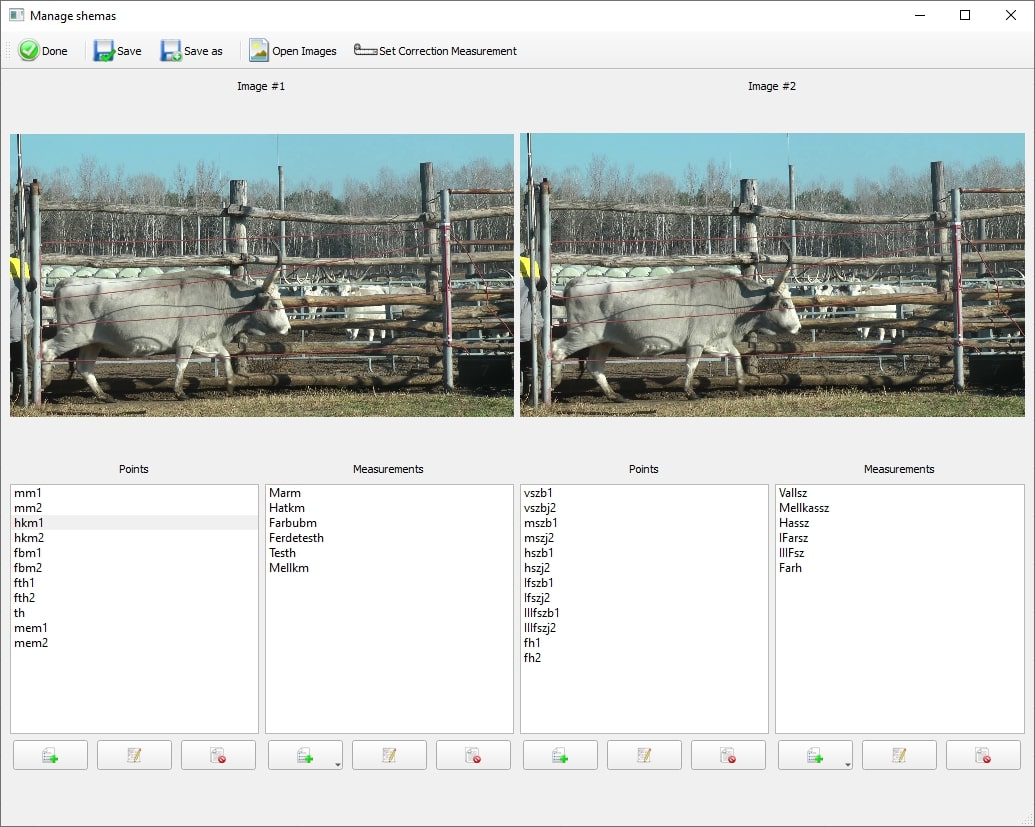
\includegraphics[width=0.95\textwidth]{./images/SchemW.jpg}
	\end{subfigure}
	\caption[]
	{\small  The Schema Window.}
\end{figure} 

\subsection{Open images}

Once a schema is open, you can open existing still images to assist with the visualization of your points and measurement. Note, that this feature only server as a visual aid, and has no actual effect on the schema or the measurement. Just like the still opening feature, you will get a pop-up file selection dialog for each camera.

\subsection{Points}

The next step is adding marker points to the schema. These points are the markers you will have to locate on the created stills in a later phase. You can define these marker points separately for each camera. To add a new point, click the \textit{New Point} \img{../VAM/Icons/1462036180_list-add.png} button of the corresponding camera, and name the point. Then, click on the highlighted image to select a location of the point for visualization. Note, that this last step has no actual effect on the schema, it is only for aiding the user visually. Once created, points can be renamed and removed by selecting them from the list, and clicking the appropriate button.

\begin{figure}[H]
	\centering
	\begin{subfigure}{\textwidth}
		\centering 
		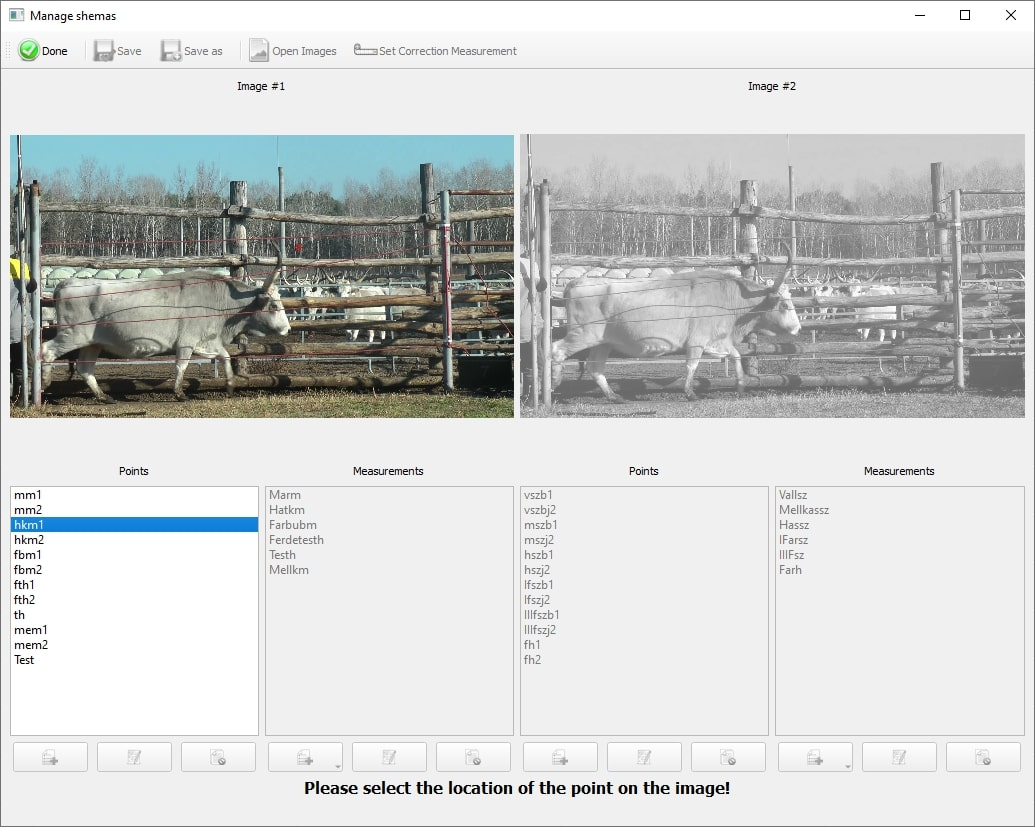
\includegraphics[width=0.95\textwidth]{./images/SchemPoint.jpg}
	\end{subfigure}
	\caption[]
	{\small  Point Creation.}
\end{figure} 

\subsection{Measurements}

The points defined in the previous step can be used to define \textit{Measurements}. Measurements have two types: \textit{Distance} measurements, requiring two points, and \textins{Angle} measurements, requiring three. To add a new measurement, click the \textit{Add} \img{../VAM/Icons/1462036180_list-add.png} button of the selected camera, and select the desired measurement type from the drop-down menu. Then, you will be prompted to select the points making up the measurement from the corresponding list. As you select the points, the visual aid interface at the top of the window will show your measurement. 

\begin{figure}[H]
	\centering
	\begin{subfigure}{\textwidth}
		\centering 
		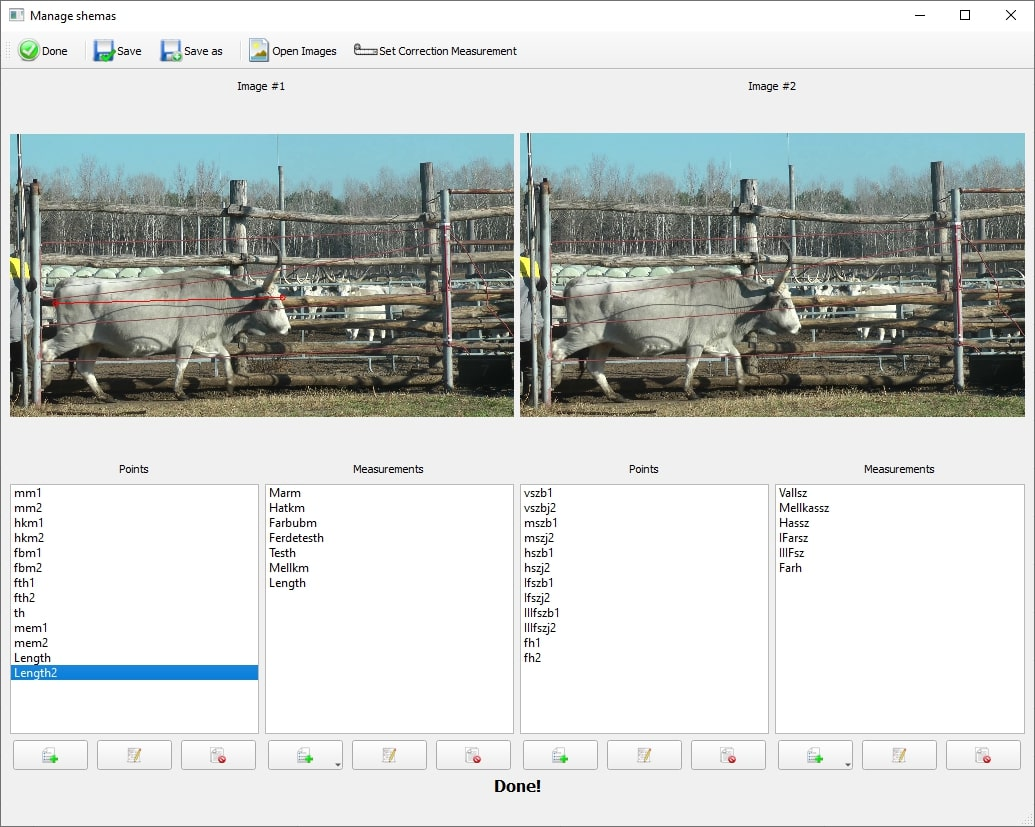
\includegraphics[width=0.95\textwidth]{./images/SchemDist.jpg}
	\end{subfigure}
	\caption[]
	{\small  Measurement Creation.}
\end{figure} 

You can also rename and delete measurements by selecting them from the list a clicking the appropriate button.

\subsection{Correction Measurement}

The final feature of  the \textbf{Schema Window} is setting the correction measurement for the \textins{Automatic Measurement Correction} setting. This feature aims to correct the issue when the etalon and the animal are not the same distance from the camera on some videos. In some of these cases, the measurement can be corrected by using the size of the animal.

\textbf{Example:} In the following example, we use two cameras to measure cattle: The first camera is looking at the animals from the side, while the second one is above the animals. The etalon on the second camera was placed on the ground, so naturally, the back of the animals is going to be significantly closer. To correct for this, the \textit{Cattle Height} measurement from camera \# 1 is selected to tell the software how much closer the given animal is to the camera compared to the etalon.

To select a correction measurement, first click the button in the toolbar, then select the camera you wish to correct. Then, select one of the measurements from the previous cameras. \textbf{NOTE:} The software can only correct \textbf{forward}, meaning the measurement correcting a particular camera has to be on one of the previous cameras.

\begin{figure}[H]
	\centering
	\begin{subfigure}{\textwidth}
		\centering 
		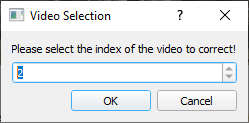
\includegraphics[width=0.25\textwidth]{./images/SelectVideoCorr.png}
	\end{subfigure}
	\caption[]
	{\small  Selecting the video to be corrected.}
\end{figure} 

\section{Measurement}

The penultimate stage of the basic usage is creating the measurement. A measurement file contains all the point locations for all animals. The \textbf{Project Window} allows you to create a new measurement by clicking the appropriate button, and selecting the schema to use. A single measurement can only use one schema, so if you wish to measure the same animals using multiple schemas, then create a new measurement for each schema. You can also rename or remove measurement. 

\begin{figure}[H]
	\centering
	\begin{subfigure}{\textwidth}
		\centering 
		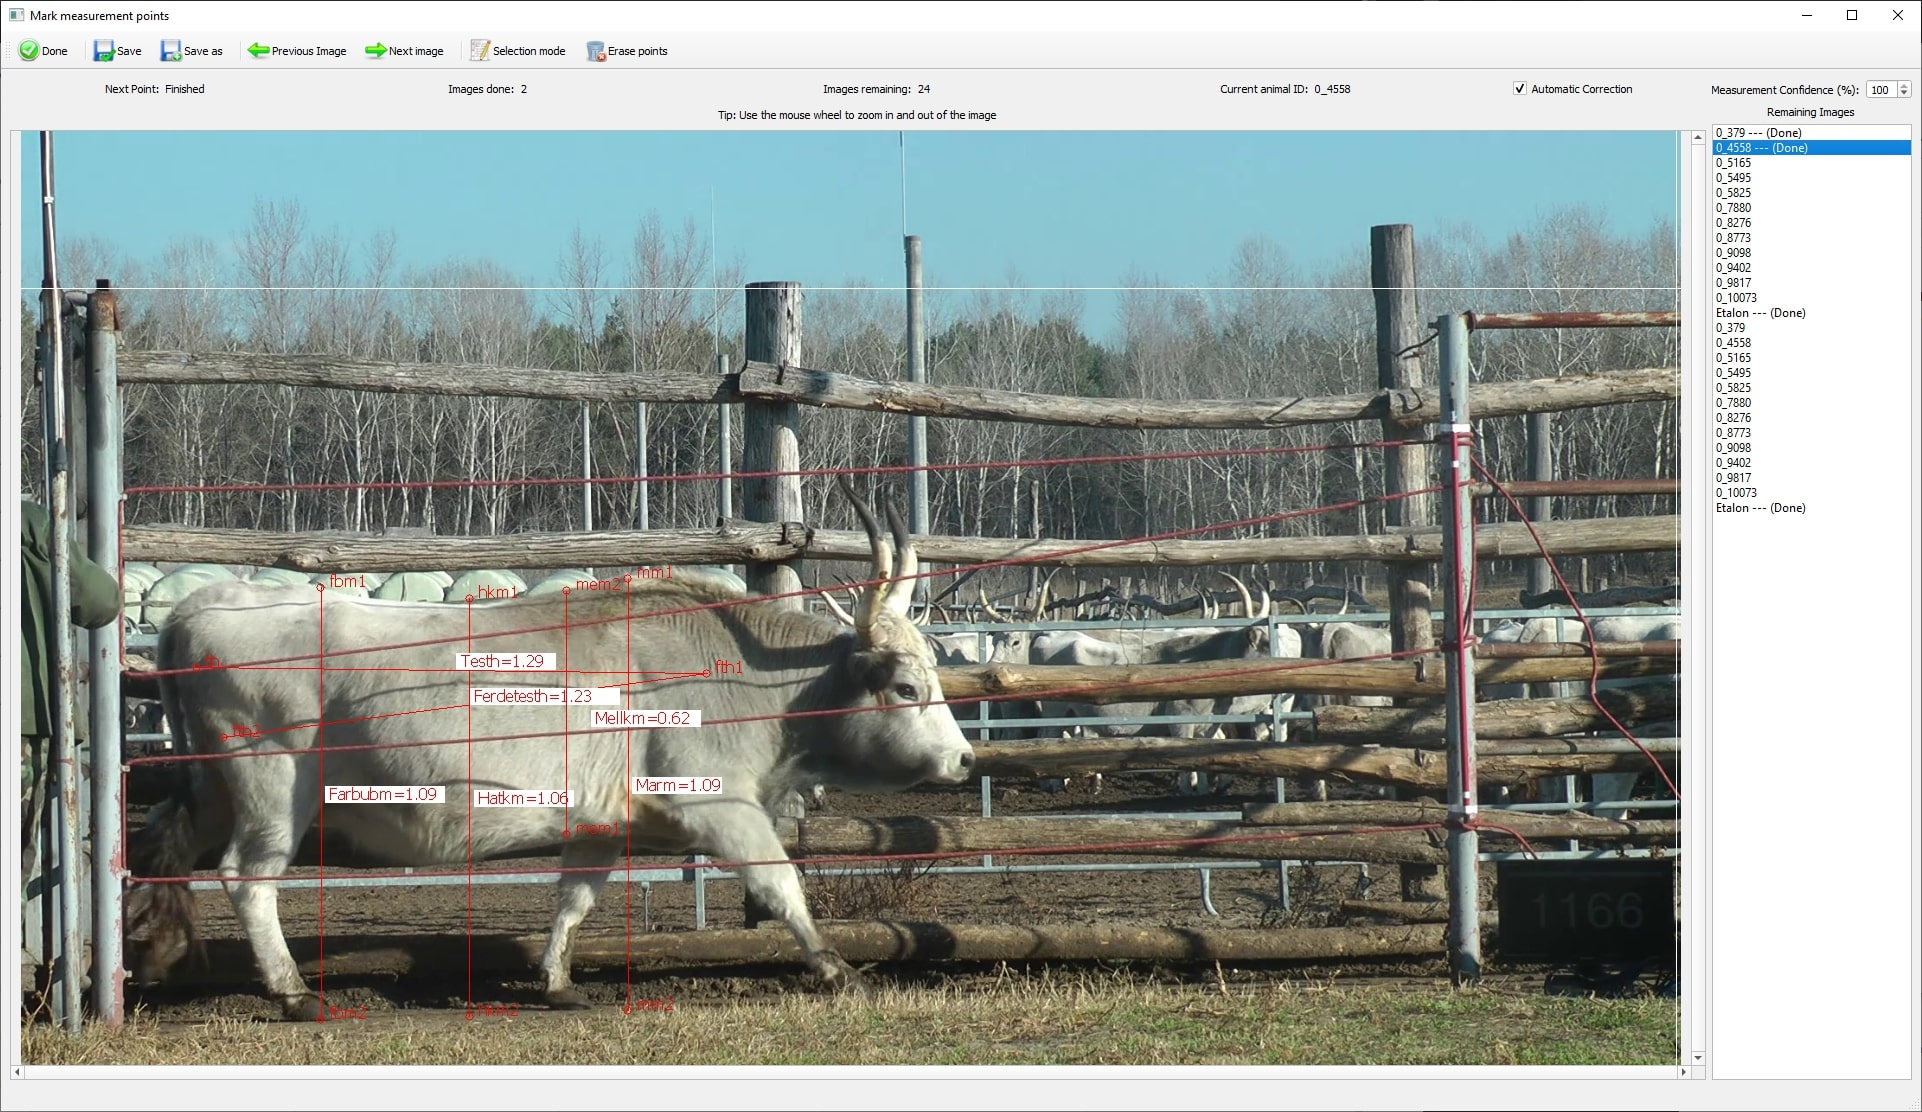
\includegraphics[width=0.95\textwidth]{./images/MeasW.jpg}
	\end{subfigure}
	\caption[]
	{\small  The Measurement Window.}
\end{figure} 

\subsection{Navigation among images}

In the \textbf{Measurement Window}, you can navigate among all the still images in the project by either using the arrow buttons (\img{../VAM/Icons/1462036195_arrow-left1.png} \img{../VAM/Icons/1462036198_arrow-right1.png}), or by double-clicking the desired still in the right side list.


\subsection{Add points}

If the \textit{AI marker} feature is enabled, then navigating to a new image will automatically result in the AI attempting to mark it, unless it is an etalon image, or if it has already been marked. \textbf{NOTE: The VATEM3 software currently only supports automatically marking cattle images, where camera \# 1 is  a side image and camera \# 2 is a top image. The schema also has to match the following definition.}

\textbf{If any of these conditions is not met, then the AI-assisted marker placement will be automatically disabled.}

If you choose manual marking, then you can do that by simply clicking the image where you want to place the markers. The top toolbar of the window will display the name of the point you are about to place. If the automatic marker has been completed before, you will have to erase the points to put down new ones. Alternatively, you can choose to edit the points already placed.

\subsection{Edit points}

To edit points, you have to first toggle selection mode, using the toolbar. Then you can select individual points by clicking near them. You can move the selected point by using the \textbf{<w,a,s,d>} keys, or delete it.


\begin{figure}[H]
	\centering
	\begin{subfigure}{\textwidth}
		\centering 
		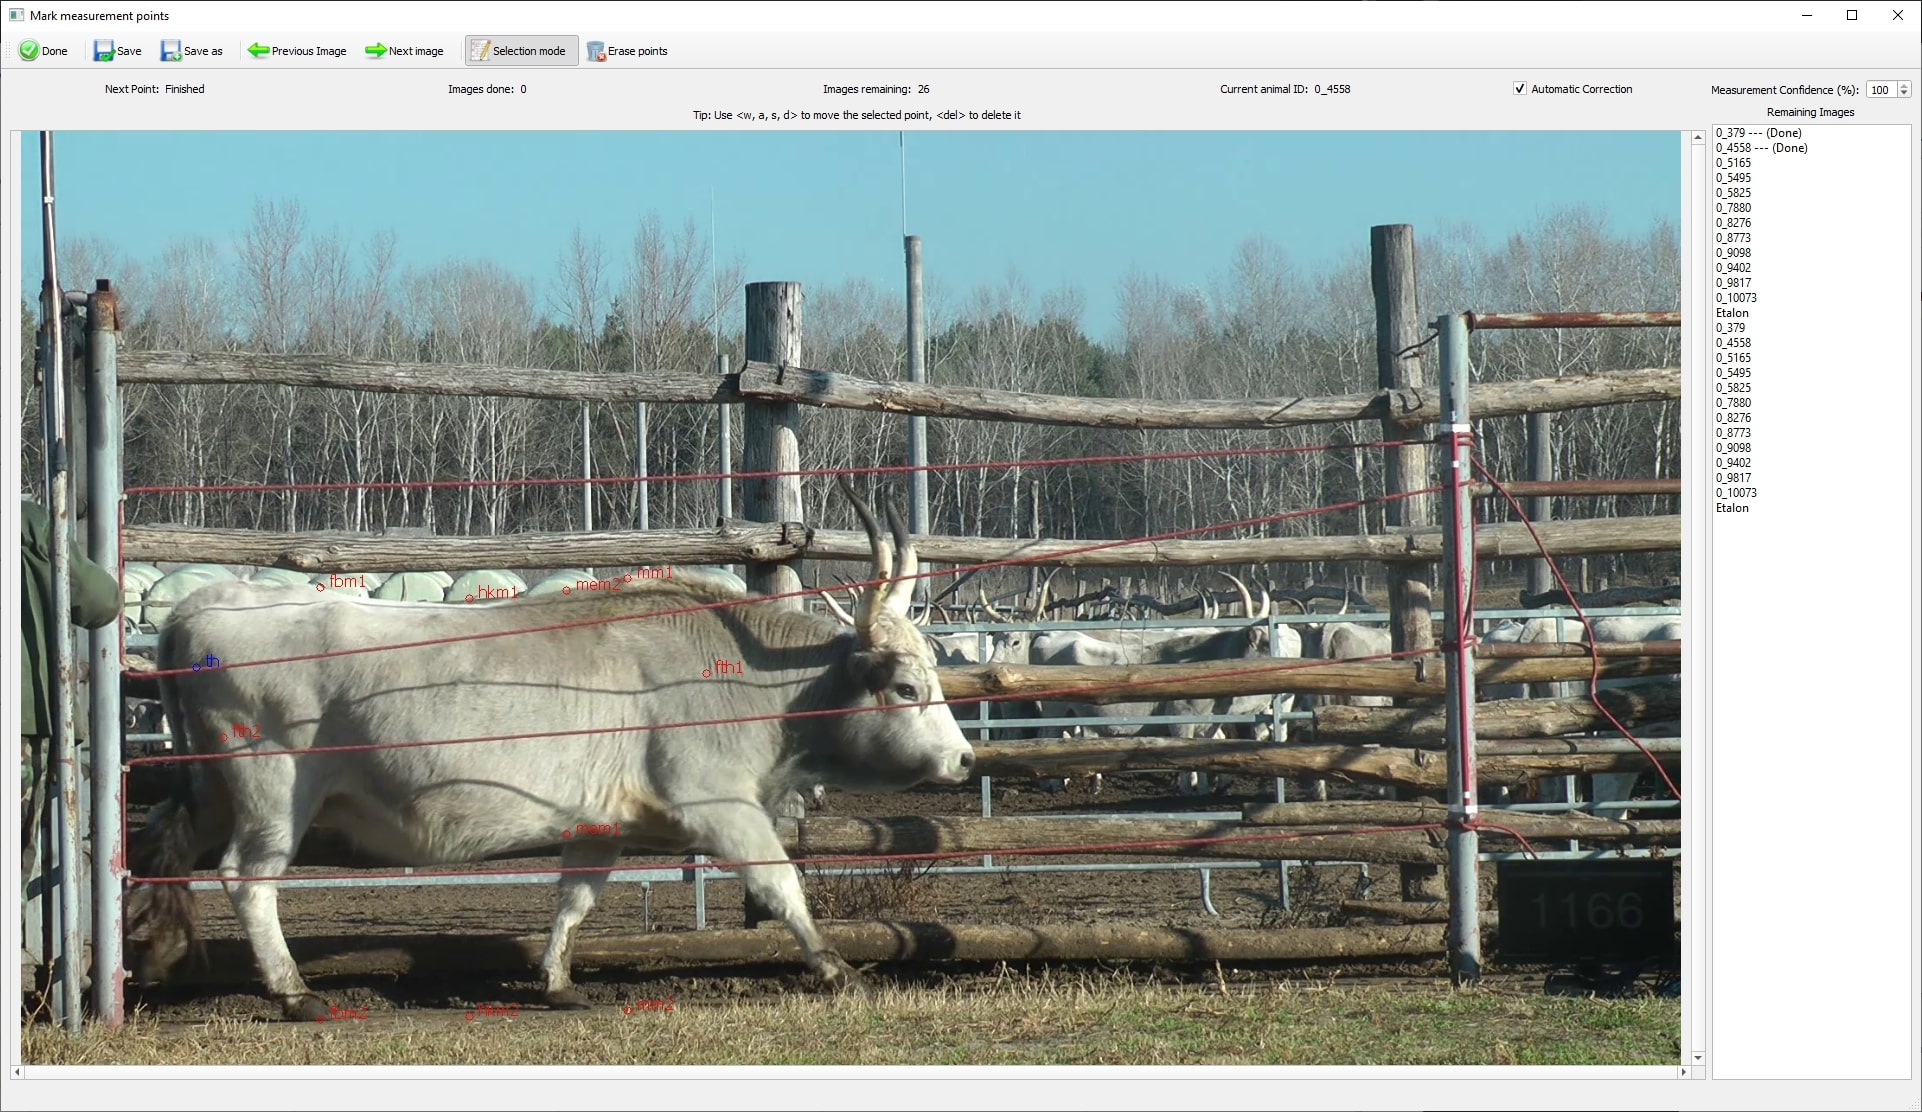
\includegraphics[width=0.95\textwidth]{./images/MeasWSel.jpg}
	\end{subfigure}
	\caption[]
	{\small  Editing marker points.}
\end{figure} 

You can also set the measurement confidence for each still separately, which will be saved to the report file.

\section{Output generation}

The final stage of the project lifecycle is output generation. In this stage, you can save your measurement data by selecting a desired format from the drop-down list, and hitting \textit{Generate}. Once the progress bar is finished, your output files will be found in the \textit{"<Project Folder>/Outputs"} folder.


\begin{figure}[H]
	\centering
	\begin{subfigure}{\textwidth}
		\centering 
		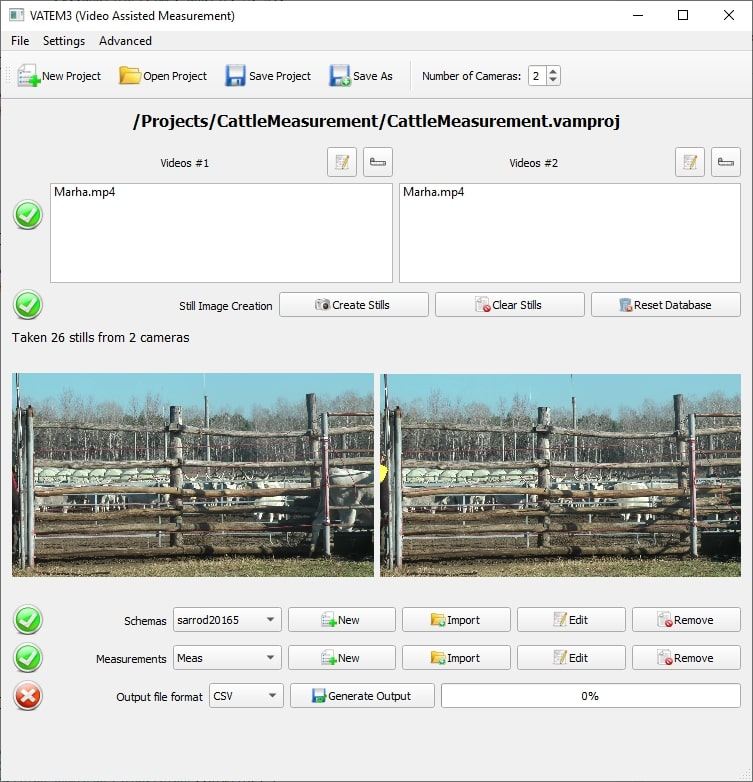
\includegraphics[width=0.75\textwidth]{./images/MWFin.jpg}
	\end{subfigure}
	\caption[]
	{\small  A finished project.}
\end{figure} 

\subsection{Formats}

VATEM3 currently supports 3 formats: raw cvs, xlsx and html. The first simply saves all measurement data for each animal in a comma separated values file, which is ideal for any future automatic processing step. The xlsx format saves the same data, but in a more human-readable and editable form. The html format generates a report that includes the completed measurement images as well, and is the most readably of the there formats. 

NOTE: The measurement images are saved next to the output file in all three cases.


\chapter{Advanced Usage}

In this chapter, we cover the more advanced features of the VATEM3 software, namely \textbf{Camera Calibration, Automatic Still Generation, Planimetrics} and \textbf{Morphometrics}.

\section{Calibration}

The camera calibration function can be used to avoid two practical problems with commercial video cameras: Non-square pixels and geometric distortion. The first issue mostly occurs in old video cameras, and results in incorrect measurements, as the VATEM3 software assumes that the cameras have square-shaped pixel sensors. The second causes "barrel" and "pillow" distoritons in the image, causing straight lies to curve in the image. \textbf{NOTE: If your camera does not have these issues, then Calibration is completely unnecessary, and may cause inaccurate measurements.}

You can perform calibration for each camera, click the \textit{Calibrate} \img{../VAM/Icons/1462455465_centimeter.png} button in the \textbf{Video Stage} of the \textbf{Project Window}. This will launch a calibration wizard, which asks you to print an image of a chessboard calibration object on a A4 size paper. After printing the image, secure it on a flat, rigid surface to prevent the paper from folding, as that will give your very inaccurate results.

\subsection{Take video}

The second step of calibration is to record a short video with your camera, where you show the calibration object from multiple angles and distances. Make sure that your video contains plenty of frames, where the calibration object is fully visible, and sharp. Try to include as many angles and distances as you can, and make sure the calibration object is not always perfectly in the middle of the image. See below a few important positions you will need. 

\subsection{Perform calibration}

Once the video is done, save it on your computer, and load it in the next window of the wizard. Once the video is loaded, adjust the settings if necessary, and hit calibrate. Please be aware that if the recorded video is not good quality then this feature (especially the estimation of distortion) may cause more harm than good.

\begin{figure}[H]
	\centering
	\begin{subfigure}{\textwidth}
		\centering 
		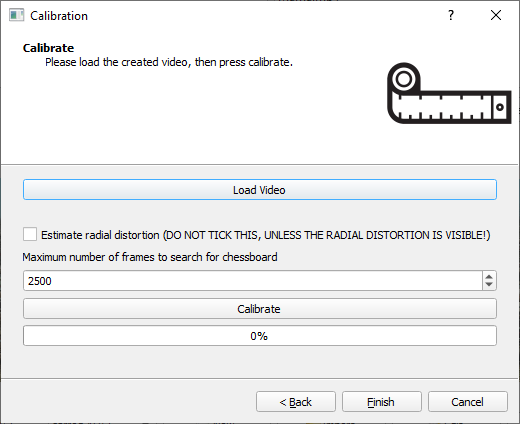
\includegraphics[width=0.5\textwidth]{./images/Calib.png}
	\end{subfigure}
	\caption[]
	{\small  The Calibration Wizard.}
\end{figure} 

\section{Automatic still generation}

Another advanced feature is AI assisted automatic still image generation, accessible from the \textbf{Still Window}. Currently, the software only supports the detection of cattle in side and top images.

You can access this feature by clicking the \textit{Automatic Detection} button.

\begin{figure}[H]
	\centering
	\begin{subfigure}{\textwidth}
		\centering 
		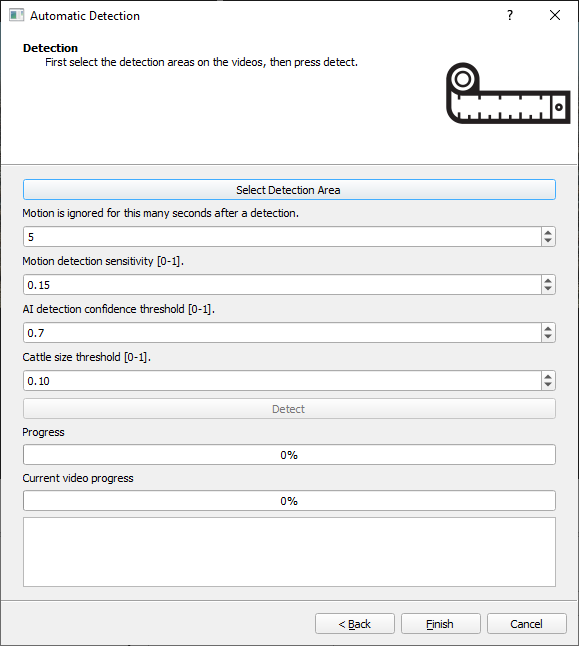
\includegraphics[width=0.5\textwidth]{./images/AutoDetect.png}
	\end{subfigure}
	\caption[]
	{\small  The Detection Wizard.}
\end{figure} 

\subsection{Set detection area}

You first task in the wizard is to select the detection area. To achieve higher speeds, the software runs motion detection in this area to pic out frames it needs to investigate further. You can select the area by drawing a rectangle on the images with your mouse. 

\textbf{NOTE: The detection area should encompass the full height of the animals, and roughly 50\% of the length of the area where they are visible. The area should be on the opposide side from where animals enter! This ensures that once an animal enters the detection area, they are already fully visible in the image. See examples below.}

\begin{figure}[H]
	\centering
	\begin{subfigure}{\textwidth}
		\centering 
		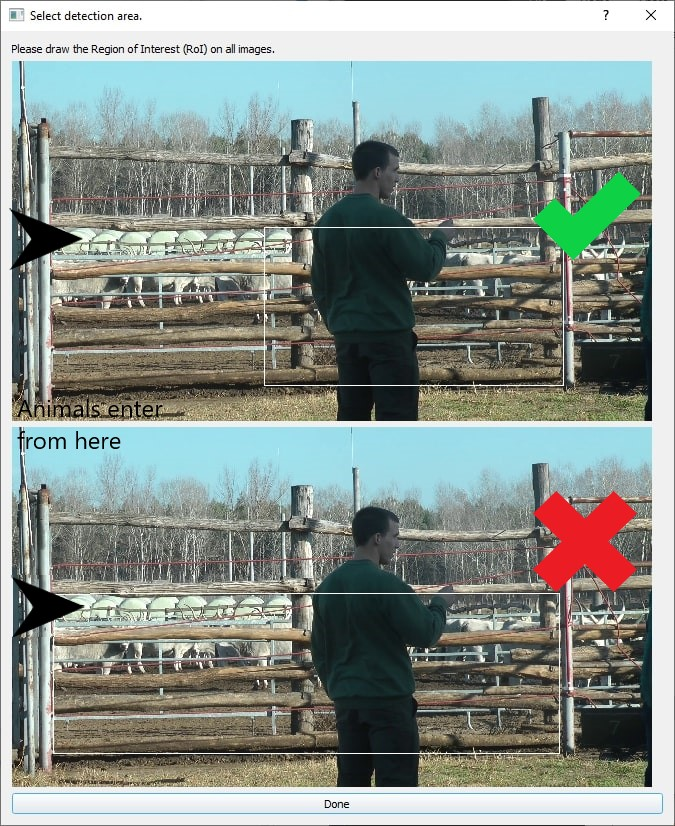
\includegraphics[width=0.5\textwidth]{./images/DetArea.jpg}
	\end{subfigure}
	\caption[]
	{\small  Setting the detection area: Top image is correct, BOTTOM MAGE SHOWS INCORRECT AREA!}
\end{figure} 

\subsection{Detection}

The detection process has multiple adjustable settings. The first one is the \textbf{Motion Detection Delay}, which defines a time period after a motion detection, when the algorithm ignores any further motion events. This ensures that the same animal is not detected multiple times. The second setting is the \textbf{Motion Threshold}, which controls the sensitivity of  the motion detection. The higher this setting, the less sensitive the algorithm becomes. 

The next setting is the \textbf{Confidence Threshold}, which is the sensitivity of the AI-based cattle recognition. The higher this setting, the more certain the AI needs to be that it has seen a cattle. The last setting is the \textbf{Area Threshold}, which sets the minimum area an animal needs to be to count as a detection. This setting aims to avoid accidentally detecting cattle in the background.

Once the settings are set, you can launch the detection. Once the detection is finished, you can launch a dialog to pair and add the detected still images (see: \autoref{sec:openStill, sec:compStill}).

\begin{figure}[H]
	\centering
	\begin{subfigure}{\textwidth}
		\centering 
		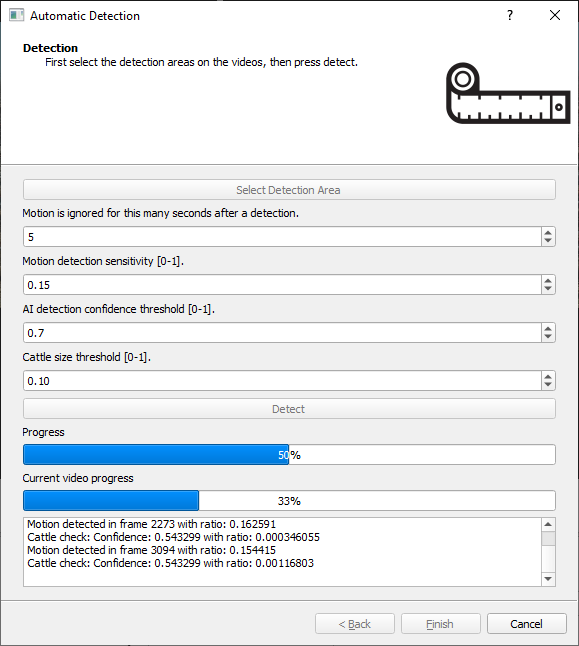
\includegraphics[width=0.5\textwidth]{./images/AutoDetect2.png}
	\end{subfigure}
	\caption[]
	{\small  Detection in progress.}
\end{figure} 

\section{Planimetrics}

The next advanced feature of the VATEM3 software is the \textbf{Planimetrics }export. This feature allows users to mark the area belonging to the animal in the images and export accurate segmentation data on all animals for future processing. To launch planimetrics, use the corresponding item in the \textit{Advanced} menu of the \textbf{Project Window}.

This feature also supports estimating animal weight measurement by assuming a proportional relationship between animal area and weight. You can set the area-to-weight ratio in the upper toolbar of this window. 

The upper toolbar also allows you to navigate between images using the arrow keys, or clear images and export the final planimterics data. 

The \textbf{Planimetrics Window} provides several powerful tools to allow you to perform manual segmentation and semi-automatic segmentation quite easily. All tools allow you to mark areas as animal by default, or mark them as background, if the \textit{Erase Mode} option is toggled.

\subsection{Polygon tool}

The polygon tool allows you to draw polygon shapes onto the image. To do this, make sure, that \textins{Polygon} is selected from the drop-down list on the left, then proceed to put down the outer corners of the polygon onto the image by clicking on it. Once finished, click the \textit{Draw Polygon} button. You can put down multiple polygons.


\begin{figure}[H]
	\centering
	\begin{subfigure}{\textwidth}
		\centering 
		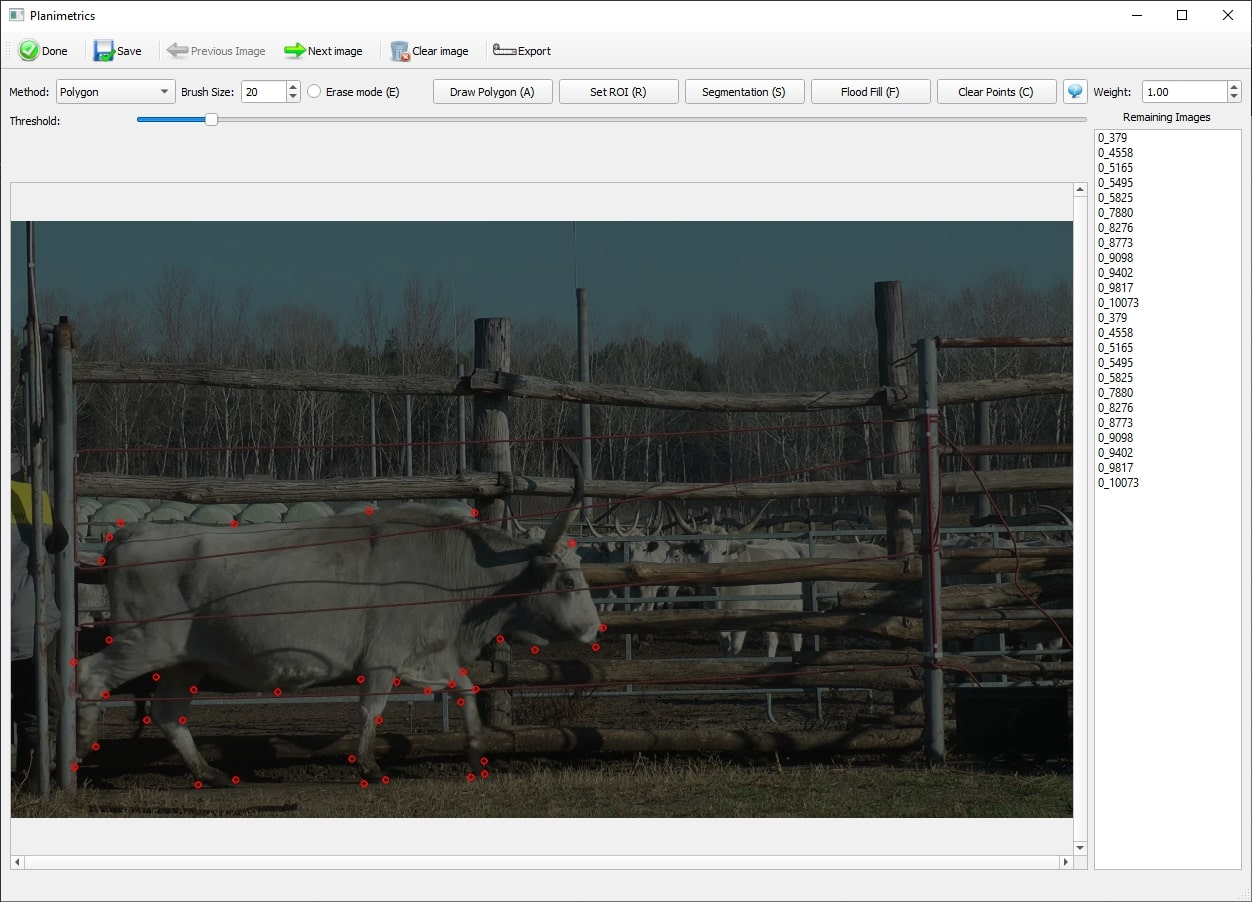
\includegraphics[width=0.95\textwidth]{./images/PlaniPoly1.jpg}
	\end{subfigure}
	\begin{subfigure}{\textwidth}
	\centering 
	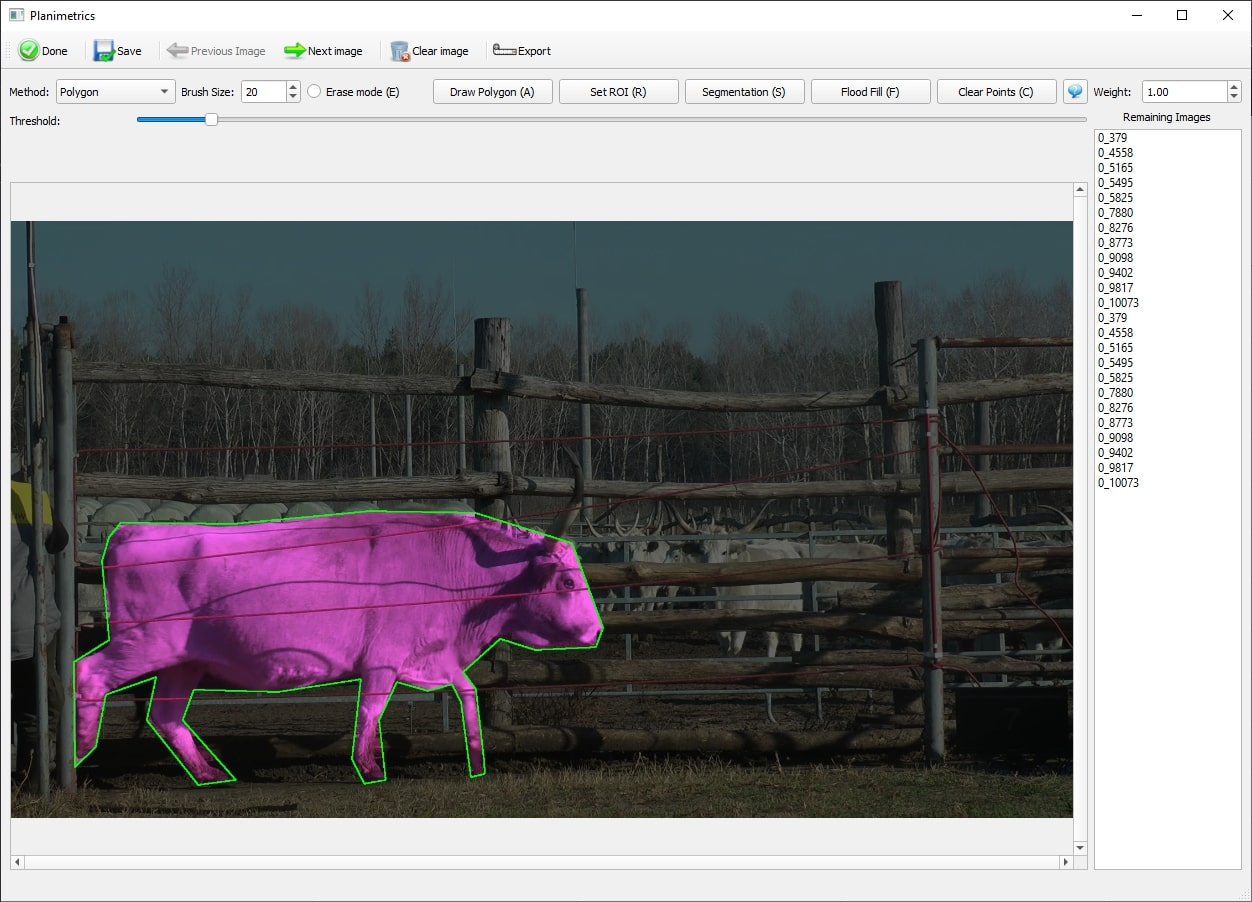
\includegraphics[width=0.95\textwidth]{./images/PlaniPoly2.jpg}
	\end{subfigure}
	\caption[]
	{\small  Using the polygon tool.}
\end{figure} 

\subsection{Automatic segmentation}

You can also perform automatic segmentation by selecting a \textbf{Region of Interest (RoI)} on the image. To do this, put down at least 2 point on the image using the polygon tool. These two points will define a rectangle. Once finished, click the \textit{Set ROI} button, then click on the \textit{Segmentation} button. By changing the threshold slider, you can increase or decrease the sensitivity of the segmentation.

Another way of automatic segmentation is by flood filling the image from a certain point. To do this, set a ROI as before, and click the \textit{Flood Fill} button. Then click the image at the location you want to start the flooding, and change the threshold slider to get close to the desired result.

\begin{figure}[H]
	\centering
	\begin{subfigure}{\textwidth}
		\centering 
		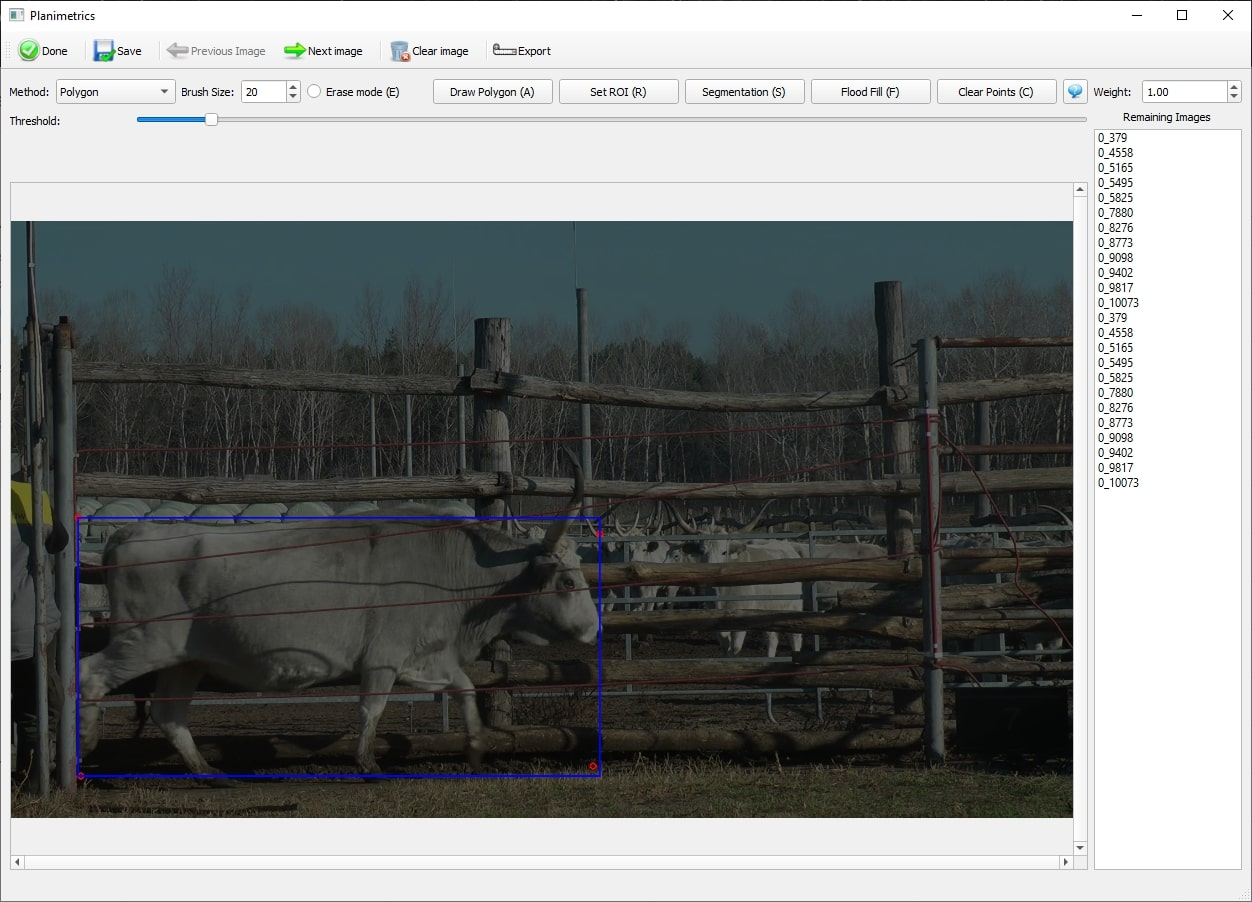
\includegraphics[width=0.95\textwidth]{./images/PlaniROI.jpg}
	\end{subfigure}
	\begin{subfigure}{\textwidth}
		\centering 
		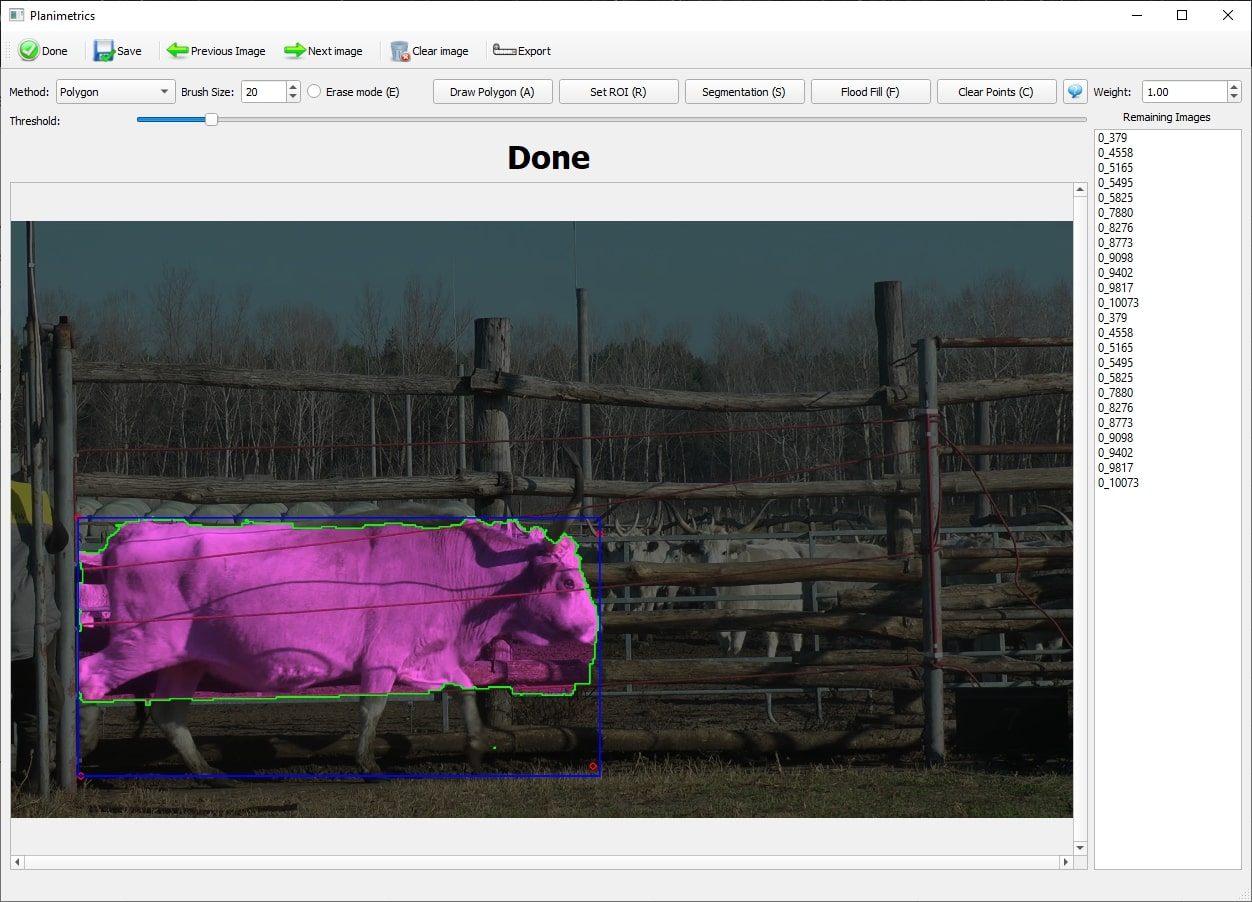
\includegraphics[width=0.95\textwidth]{./images/PlaniSeg.jpg}
	\end{subfigure}
	\caption[]
	{\small  Using the automatic segmentation tool.}
\end{figure} 

\subsection{Brush tools}

The final set of tools allow you to make minor corrections to the segmentation mask. To use these, select the \textit{Circular Brush} or the \textit{Rectangular Brush} tools from the drop-down list. Then you can set the size of these tools using the spin box next to the list. Finally, by clicking on the image the brush adds or erases the covered area from the segmentation mask, depending on the \textit{Erase Mode} setting.

\section{Morphometrics}

The final advanced feature of the VATEM3 software is exporting Morphometric data from the measurements. To launch this feature, the project has to have completed the measurement stage. After that, this can be launched from the \textins{Advanced} menu of the \textbf{Project Window}. 

\begin{figure}[H]
	\centering
	\begin{subfigure}{\textwidth}
		\centering 
		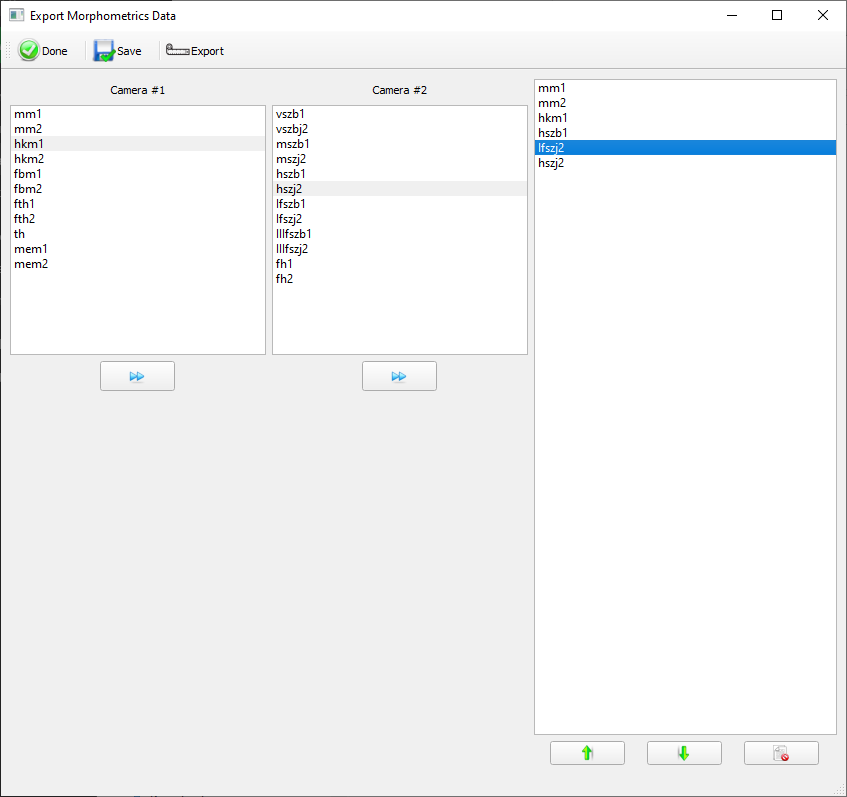
\includegraphics[width=0.5\textwidth]{./images/Morpho.png}
	\end{subfigure}
	\caption[]
	{\small  The Morphometrics Window.}
\end{figure} 

\subsection{Setup data}

Once the window is launched, you need to set up your morphometric data by adding points from all cameras to the export order. Once added, the points can be rearranged or remove entirely. Once the data format is set up, the export can be launched using the \textit{Export} button.

\chapter{Troubleshooting}

If you encounter any issues with the software, we appreciate that you submit an error report on the project's GitHub page, at \url{https://github.com/szemenyeim/VAM}. Generally, it is advisable to adhere to the following guidelines:

\begin{enumerate}
	\item Although all project files are editable in text editors, we strongly recommend not to do this.
	\item Do not move project files, videos or images in different folders after creating the project.
	\item If you open a project created on another computer, it is recommended to first copy the files to your project directory.
	\item Similarly, if you import existing files (schemas, measurement, images, etc.) into a project, it is recommended to first copy the files to your project directory.
\end{enumerate}


\section{Error reporting}

If you encounter an error, we request that you make an error report including a following information:

\begin{itemize}
	\item Type and Version of the OS
	\item Version of the VATEM3 software (shown in the About information)
	\item A detailed description of the error (unexpected behavior, error message, crash, etc.)
	\item A detailed description of your actions leading up to the error
	\item A VATEM3 log file (see the next section)
	\item The project you were working on. This includes the .vamproj and .stilldb files, as well as all .schema and .meas files imported into your project. You do not have to attach any videos or images, unless you think they are relevant to your error.
\end{itemize}

\subsection{Accessing the VATEM3 log}

To access the VATEM3 log file, you first have to turn on logging. This can be done in the \textit{Settings} menu of the \textbf{Project Window}. Once this is done, the log file will be available in your installation folder (where VATEM3.exe is also located). Attaching this file to your error report help us reproduce the issue you encountered, and thus fix it as soon as possible.

\chapter*{Declaration of Support}

Very offical BS

\nocite{*}
\printbibliography[title=Acknowledgements,heading=bibliography,keyword=0]


\label{page:last}
\end{document}